\part[Programming Paradigms]{Programming Paradigms}
\section{Semantics}
\begin{frame}{Semantic classes}
\begin{block}{What is a paradigm?}
\pause
Paradigm = Semantic class
\end{block}
\pause
\begin{block}{What does ``semantic'' mean?}
\pause
Semantics = Meaning
\end{block}
\pause
\begin{block}{What is a ``programming'' paradigm?}
\pause
Programming paradigm = semantic class of a \highlight{program}
\end{block}
\pause
\begin{block}{Is more than one programming paradigm known to mankind?}
\pause
Yes
\end{block}
\end{frame}

\begin{frame}{Semantic classes}
\begin{block}{Can two programs, which belong to different semantic classes have
same semantics?}
\pause
Yes
\end{block}
\pause
\begin{block}{Can a program belong to more than one semantic class?}
\pause
Yes
\end{block}
\pause
\begin{block}{Does a program have to belong to a semantic class at all?}
\pause
No
\end{block}
\end{frame}

\begin{frame}{Semantic classes}
\begin{block}{What purpose do semantic classes serve?}
\pause
Semantic classes make programmers think about programs differently
\end{block}
\pause
\begin{block}{How do they do it?}
By disallowing programmers to think in particular ways
\end{block}
\pause
\begin{block}{Does it help?}
\pause
Yes
\end{block}
\pause
\begin{block}{
How can one ``force'' a programmer to think according to a semantic class?}
\pause
By \alert{removing} features from the programming language he uses!
\end{block}
\end{frame}

\subsection{Modular Programming}
\begin{frame}{Modular Programming}
\begin{block}{What is Modular Programming?}
Modular Programming is  a discipline imposed on file size (program length,
\highlight{module length})
\end{block}
\pause
\begin{block}{What should you do if your program does not fit into a single
file?}
Make sure you have the ability to jump from file to file (Sounds like a
\lstinline!goto! statement)
\end{block}
\end{frame}

\subsection{Structured Programming}
\begin{frame}{Structured Programming}
\begin{block}{What is Structured Programming?}
Structured Programming is a discipline imposed upon \highlight{direct transfer
of control} (no \lstinline!goto!)
\end{block}
\pause
\begin{block}{How to meet such a constraint?}
Use only \highlight{sequence}, \highlight{selection} and
\highlight{iteration}
\end{block}
\pause
\begin{block}{What benefits do we gain?}
The ability to prove \highlight{correctness of our programs}, easiness of
reasoning about our programs (and less spaghetti code)
\end{block}
\end{frame}

\subsection{Object-Oriented Programming}
\begin{frame}{Object-Oriented Programming}
We want to write a program, which copies characters from the
\highlight{keyboard} to the \highlight{printer}
\end{frame}

\begin{frame}[fragile]{Object-Oriented Programming}
\begin{lstlisting}[language=c]
void copy() {
   int c;
   while((c = readKeyboard()) != EOF) {
      writePrinter(c);
   }
}
\end{lstlisting}
\end{frame}

\begin{frame}{Object-Oriented Programming}
Now we want to modify our program, so that it sometimes reads characters
from the \highlight{keyboard} and sometimes reads characters from the
\highlight{paper tape reader} and writes them to the \highlight{printer}
\begin{center}
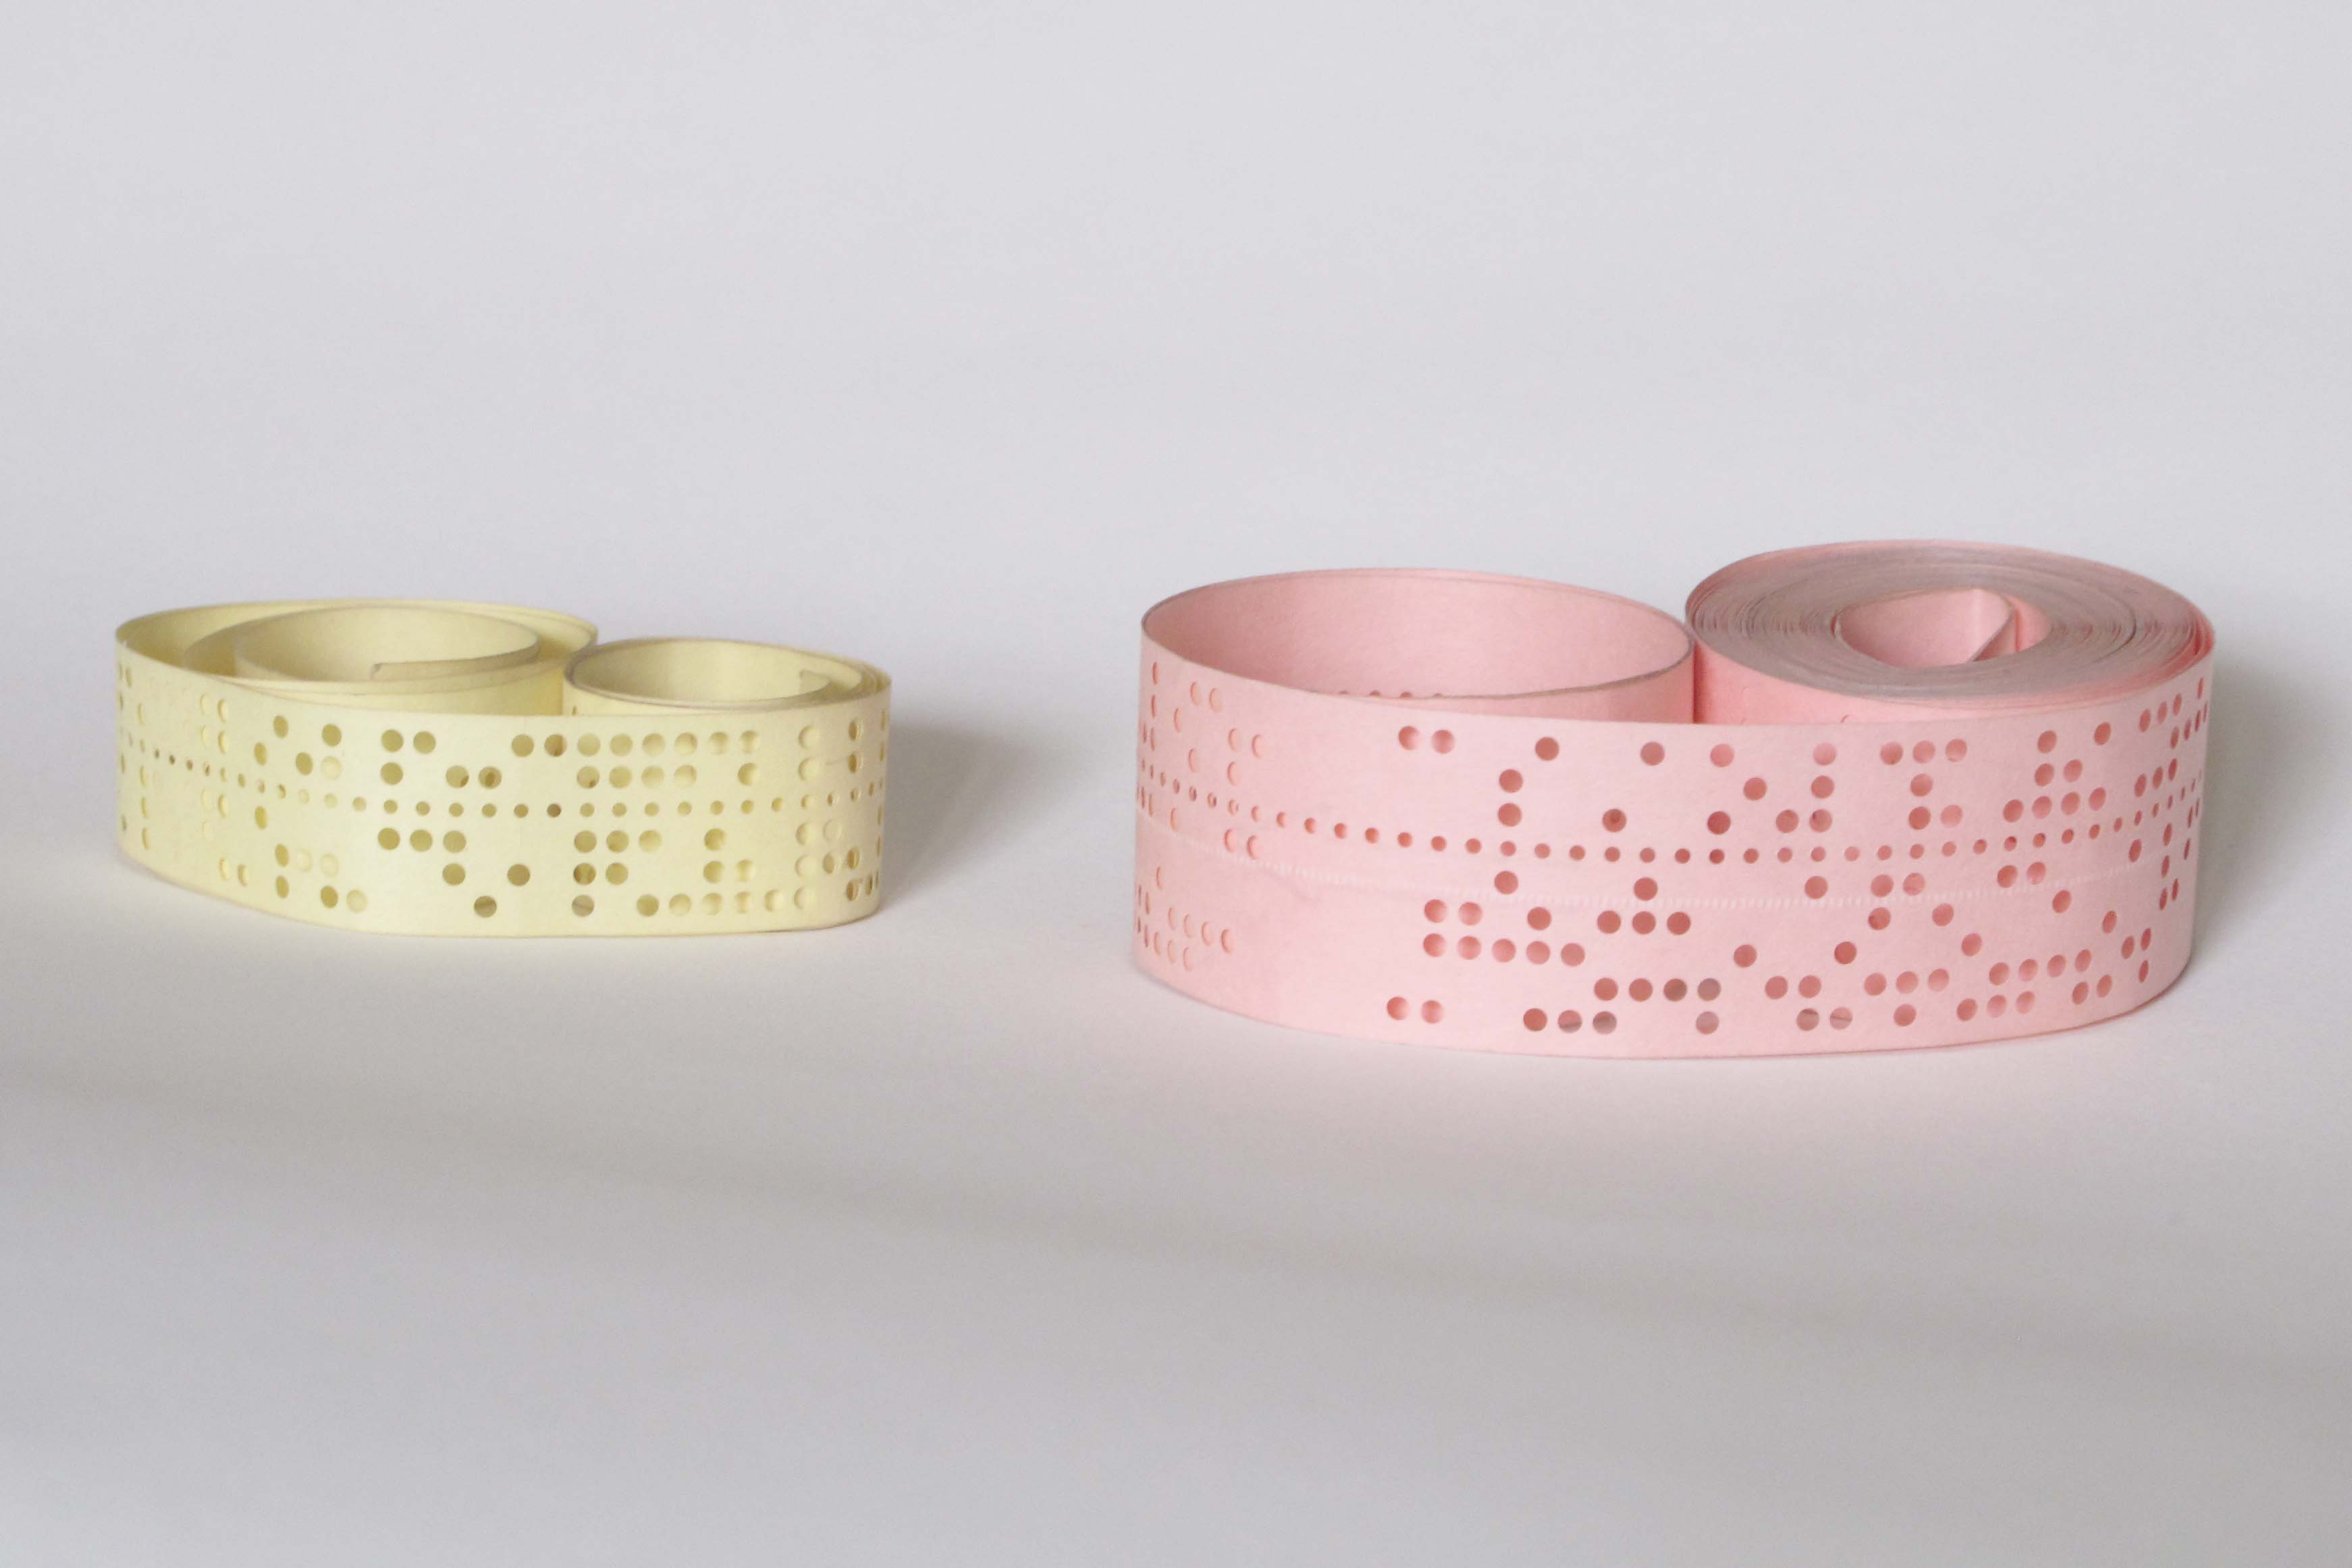
\includegraphics[width=0.5\textwidth]{resources/PaperTapes.jpg}
\end{center}
\end{frame}

\begin{frame}[fragile]{Object-Oriented Programming}
\begin{lstlisting}[language=c]
bool GptFlag = false;
// Remember to clear

void copy() {
   int c;
   while((c = (GptFlag ? readPt() : readKeyboard())) != EOF) {
      writePrinter(c);
   }
}
\end{lstlisting}
\end{frame}

\begin{frame}{Object-Oriented Programming}
Now we want to modify out program, so that it sometimes reads characters
from the \highlight{keyboard} and sometimes reads characters from the
\highlight{paper tape reader} and writes them sometimes to the
\highlight{printer} and sometimes to the \highlight{paper tape punch}
\end{frame}

\begin{frame}[fragile]{Object-Oriented Programming}
\begin{lstlisting}[language=c]
bool GptFlag = false;
bool GpunchFlag = false;
// Remember to clear

void copy() {
   int c;
   while((c = (GptFlag ? readPt() : readKeyboard())) != EOF) {
      GpunchFlag ? writePunch(c) : writePrinter(c);
   }
}
\end{lstlisting}
\end{frame}

\begin{frame}{Object-Oriented Programming}
\begin{center}
Each time we add \highlight{new devices} our code becomes \alert{less
maintainable}.\\
Let us take a look at the \highlight{diagrams} to find out why\ldots
\end{center}
\end{frame}

\pictureframe{{Object-Oriented Programming}}{resources/OO1.pdf}
\pictureframe{{Object-Oriented Programming}}{resources/OO2.pdf}

\begin{frame}{Object-Oriented Programming}
\begin{center}
OO to the rescue
\end{center}
\end{frame}

\begin{frame}[fragile]{Object-Oriented Programming}
\begin{lstlisting}[language=c]
void copy() {
   int c;
   while((c = getchar()) != EOF) {
      putchar(c);
   }
}
\end{lstlisting}
\end{frame}

\pictureframe{{Object-Oriented Programming}}{resources/OO3.pdf}
\pictureframe{{Object-Oriented Programming}}{resources/OO4.pdf}

\begin{frame}[fragile]{Object-Oriented Programming in C (not C++)}
\begin{lstlisting}[language=c]
#include <stdio.h>

typedef void(*pointerToFunction)();
\end{lstlisting}
\pause
\begin{lstlisting}[language=c]
typedef struct {
   pointerToFunction memberFunction;
} Base;
\end{lstlisting}
\pause
\begin{lstlisting}[language=c]
typedef struct {
   pointerToFunction memberFunction;
} Derived;
\end{lstlisting}
\pause
\begin{lstlisting}[language=c]
void derivedFunctionImplementation() {
   printf("Hello from derived");
}
\end{lstlisting}
\end{frame}

\begin{frame}[fragile]{Object-Oriented Programming in C (not C++)}
\onslide<1->\begin{lstlisting}[language=c]
int main(int argc, char* argv[]) {
\end{lstlisting}
\onslide<2->\begin{lstlisting}[language=c]
   Derived derived;
   Base* basePointer;

\end{lstlisting}
\onslide<3->\begin{lstlisting}[language=c]
   // mimicing a class method
   derived.memberFunction = derivedFunctionImplementation;
   
\end{lstlisting}
\onslide<4->\begin{lstlisting}[language=c]
   // polymorphic binding at runtime
   basePointer = (Base*) &derived;

\end{lstlisting}
\onslide<5->\begin{lstlisting}[language=c]
   // polymorphic invocation of derivedFunctionImplementation
   basePointer -> memberFunction();
\end{lstlisting}
\onslide<1->\begin{lstlisting}[language=c]
}
\end{lstlisting}
\end{frame}

\begin{frame}[fragile]{Object-Oriented Programming}
\begin{block}{What is the meaning of the difference between\ldots}
the \highlight{procedural}\\
\begin{lstlisting}
f(o, x)
\end{lstlisting}
and the \highlight{OO} notations?
\begin{lstlisting}
o.f(x)
\end{lstlisting}
\end{block}
\end{frame}

\pictureframe{{Object-Oriented Programming}}{resources/OO5.pdf}

\begin{frame}{Object-Oriented Programming}
\begin{block}{What is Object-Oriented Programming?}
Object-Oriented Programming is a discipline imposed upon \highlight{indirect
transfer of control} (no pointers to functions)
\end{block}
\pause
\begin{block}{How to meet such a constraint?}
Use \highlight{polymorphism} to manage dependencies
\end{block}
\pause
\begin{block}{What benefits do we gain?}
The easy ability to structure our modules so that the source code dependencies
oppose the flow of control
\end{block}
\end{frame}

\subsection{Functional Programming}
\begin{frame}{Functional Programming}
\begin{block}{What is Functional Programming?}
Functional Programming is a discipline imposed upon \highlight{mutability} (no
assignment)
\end{block}
\pause
\begin{block}{How to meet such a constraint?}
Embrace \highlight{immutability} and \highlight{manage mutable state}
\end{block}
\pause
\begin{block}{What benefits do we gain?}
Deterministic concurrent programming and even more easiness of
reasoning about our programs
\end{block}
\end{frame}

\section{Programs VS Languages}
\begin{frame}{Programs VS Languages}
\begin{block}{What does it mean for a language to follow a paradigm?}
The fact, that the programming language \alert{disallows} you to write programs
in particular programming \highlight{styles}, thus \highlight{constrains} you to
program according to one or more \highlight{semantic classes} means that this
language follows certain \highlight{paradigms}
\end{block}
\pause
\begin{alertblock}{What does not it mean for a language to follow a paradigm?}
The fact, that the programming language allows you to write programs in
particular programming \highlight{style} does not mean that this language
follows a \highlight{paradigm}
\end{alertblock}
\end{frame}

\begin{frame}{Programs VS Languages}
\begin{block}{Definitions}
Languages, which follow more than one paradigm are called \highlight{hybrid}\\
Languages, which follow their paradigms \highlight{to the letter} are called
\highlight{pure}\\
\end{block}
\pause
\begin{alertblock}{Rumors}
\begin{enumerate}
\item a language is \highlight{pure} when it follows \alert{only one} semantic
class
\item \highlight{hybrid} languages are \alert{impure}
\end{enumerate}
\end{alertblock}
\end{frame}

\begin{frame}{Programs VS Languages}
\begin{exampleblock}{Examples of pure languages}
\begin{itemize}
  \item Java is a pure structured and OO language
  \item Scala ia a pure structured and OO language
  \item Haskell is a pure structured and functional language
\end{itemize}
\end{exampleblock}
\pause
\begin{block}{Examples of impure languages}
\begin{itemize}
  \item C++ is an impure structured and OO language
  \item Scala is an impure functional language
\end{itemize}
\pause
\end{block}
\begin{alertblock}{Examples of unstructured languages}
\begin{itemize}
  \item C
\end{itemize}
\end{alertblock}
\end{frame}

\section{Summary}
\begin{frame}{Summary}
\begin{itemize}
  \item Paradigms are \highlight{disciplines}
  \item Disciplines are about \highlight{constraints} not \alert{abilities}
  \item Structured programming is imposed upon \highlight{direct transfer of
  control}
  \item OO programming is imposed upon \highlight{indirect transfer of control}
  \item Function programming is imposed upon \highlight{mutability}
  \item \highlight{Hybrid} languages follow more than one paradigm
  \item \highlight{Pure} languages follow their paradigms as much as they can
\end{itemize}
\end{frame}